
\begin{document}
\maketitle


The method to assess Helium concentration evolution in cladding during operation - and the subsequent embrittlement of the steel -
consists in setting a system of differential equations (Bateman equations) that takes into account nuclear reactions taking place 
in the material during irradiation. Each equation describes the volumetric concentration N [atoms/\(m^3\)] rate of change in time \(dN/dt\) of 
an isotope present in the investigated material, and the total helium concentration is given by the sum of all the contributions. 
For our purpose, we are interested in all the reactions occurring in the cladding that have the effect of producing alpha particles 
(i.e. helium nuclei): the major contributors to helium production are \(\prescript{10}{}{\text{B}}\) and \(\prescript{58}{}{\text{Ni}}\) for what
concerns the thermal spectrum, while the nuclei we are interested in for the fast spectrum are the isotopes of key steel components as 
Iron, Chromium, Nickel together with Nitrogen and Boron, which are non-negligible impurities. Clearly, it's important to monitor all possible
precursors of helium producers.To every isotope \(\prescript{A}{Z}{X}\) susceptible of (n,\(\alpha\)) reaction is associated an equation describing its contribution to helium concentration: 
\[ \frac{d[He]_X(t)}{dt} = [X](t) \int_0^{\infty} \phi(E) \sigma_{(n,\alpha)}(E,X)dE \]

The concentration of each helium producer is itself described by an equation formed by source and destruction terms, accounting for the reactions the isotope in susceptible to. In our case: 

\begin{align}
\frac{d[\prescript{A}{Z}{X}]}{dt} = - \int_0^{\infty}\phi(E)\,\sigma_{(n,\alpha)}(E,\prescript{A}{Z}{X})\,[\prescript{A}{Z}{X}]\,dE \\
+ \int_0^{\infty}\phi(E)\,\sigma_{(n,\alpha)}(E,\prescript{A+4}{Z+2}{X})\,[\prescript{A+4}{Z+2}{X}]\,dE
\end{align}

To simplify the calculations it's common practice to choose to solve the equation getting rid of the integral via values of \(\sigma\) 
representative of energy intervals. In this work only two mean cross-sections are used: one for the thermal spectrum \(\sigma_{th}\) (representing energies up to 0.1 MeV) and one for the fast spectrum \(\sigma_{th}\). Following this approach, the previous equations become 

\begin{equation}
\left\{
\begin{aligned}
 \frac{d[\prescript{A}{Z}{X}]}{dt} = - \phi_{th}\,\sigma_{(n,\alpha)}^{th}(\prescript{A}{Z}{X})\,[\prescript{A}{Z}{X}]  - \phi_{f}\,\sigma_{(n,\alpha)}^{f}(\prescript{A}{Z}{X})\,[\prescript{A}{Z}{X}] \\
+ \phi_{th}\,\sigma_{(n,\alpha)}^{th}(E,\prescript{A+4}{Z+2}{X})\,[\prescript{A+4}{Z+2}{X}]\,\\
 + \phi_{f}\,\sigma_{(n,\alpha)}^{f}(\prescript{A+4}{Z+2}{X})\,[\prescript{A+4}{Z+2}{X}]\,
\\ 
 \frac{[He]_{\prescript{A}{Z}{X}}(t)}{dt} = [\prescript{A}{Z}{X}](t) ( \phi_{th} \sigma_{(n,\alpha)}^{th}(\prescript{A}{Z}{X}) + \phi_{f}\sigma_{(n,\alpha)}^{f}(\prescript{A}{Z}{X}))
\end{aligned}
\right.
\end{equation}
\bigskip
The total helium concentration is then obtained by the summations of all the \([He]_{\prescript{A}{Z}{X}}(t)\). It' been decided to limit the system to 11 variables, choosing to keep track of the following concentrations: \(\prescript{58}{}{Ni}, \prescript{59}{}{Ni},\prescript{10}{}{B},\prescript{14}{}{N},\prescript{52}{}{Cr},\prescript{56}{}{Fe}\) and their contributes to helium concentration, called \([He]_{Ni}, [He]_B, [He]_N, [He]_{Cr}, [He]_{Fe}\). The initial conditions are calculated from the weight percentages of AIM1 steel components, the cross-sections..........?.
The results of the Bateman system for the above mentioned isotopes solved with Runge-Kutta method are shown in figure\ref{He_evolution} 
% \begin{figure}
%     \centering
%     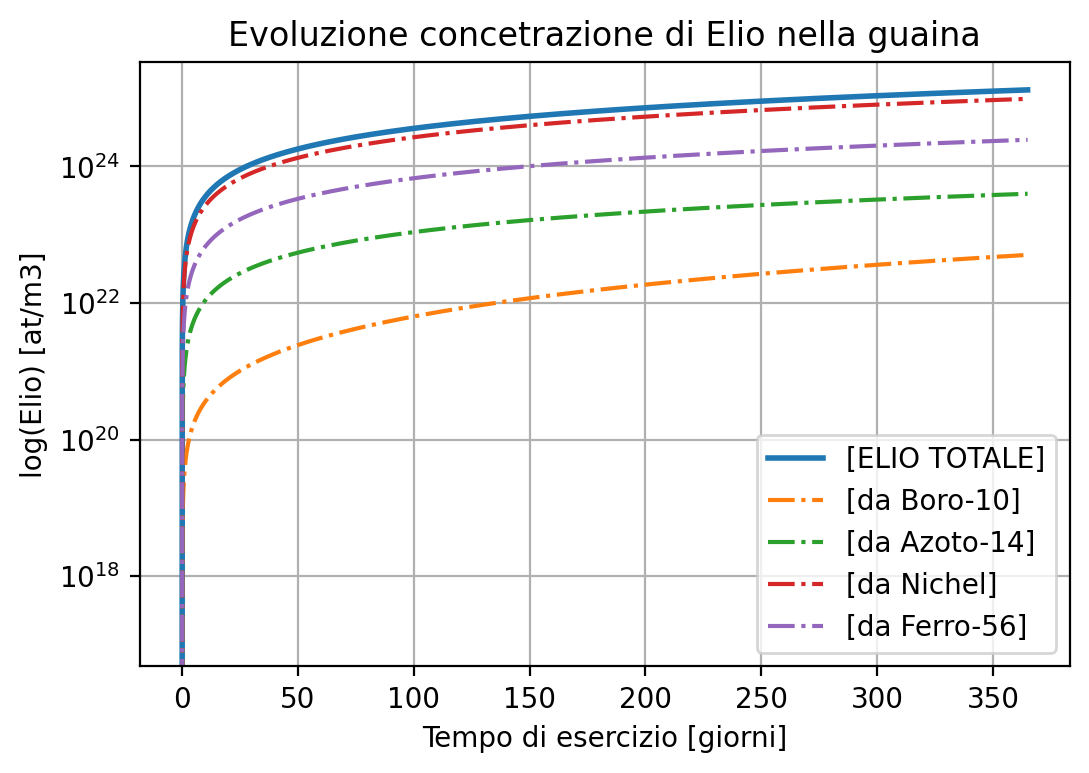
\includegraphics[width=1\linewidth]{Evoluzione Elio guaina.png}
%     \caption{Helium Concentration in cladding}
%     \label{fig:He_evolution}
% \end{figure}
\end{document}
